\begin{figure}[H]
\centering
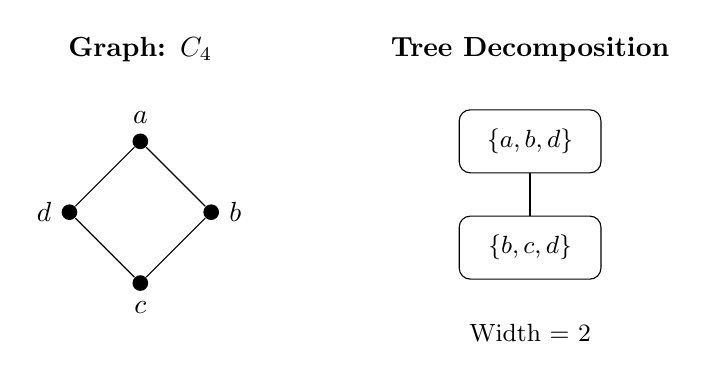
\begin{tikzpicture}[
    vertex/.style={circle,fill=black,inner sep=2pt},
    bag/.style={rectangle,draw,rounded corners,minimum width=1.8cm,minimum height=0.8cm},
    scale=0.9
]
    % Original graph - a simple cycle C4
    \begin{scope}
        \node at (0,2.8) {\textbf{Graph: $C_4$}};
        \node[vertex,label=above:$a$] (a) at (0,1.5) {};
        \node[vertex,label=right:$b$] (b) at (1,0.5) {};
        \node[vertex,label=below:$c$] (c) at (0,-0.5) {};
        \node[vertex,label=left:$d$] (d) at (-1,0.5) {};
        \draw (a) -- (b) -- (c) -- (d) -- (a);
    \end{scope}
    
    % Tree decomposition - corrected
    \begin{scope}[xshift=5.5cm]
        \node at (0,2.8) {\textbf{Tree Decomposition}};
        \node[bag] (t1) at (0,1.5) {\small $\{a,b,d\}$};
        \node[bag] (t2) at (0,0) {\small $\{b,c,d\}$};
        \draw[thick] (t1) -- (t2);
        \node at (0,-1.2) {\small Width = 2};
    \end{scope}
\end{tikzpicture}
\caption{A cycle $C_4$ and its tree decomposition of width 2}
\label{fig:tree-decomposition}
\end{figure}